\section{Simulation}\label{sec:simulation}
\subsection{Continuous prices}
In this section, we  confirm via simulations the results established analytically. We will first focus on the continuous case to mirror   Proposition \eqref{pro:finite}.  Specifically, we will demonstrate that the mean integrated square error (MISE), the square bias, and the variance of the frame-based estimator tends to zero as the number of obervations increases.  We use prices generated by 4 commonly used models of asset prices, namely, the  arithmetic Brownian motion (ABM),  the Ornstein-Uhlenbeck process (OU), the geometric Brownian motion (GBM), and the Cox-Ingersoll-Ross (CIR) process. 

We simulate prices using the following stochastic differential equations:
\begin{align}
  & X_t = 0.8 +  0.5  t + 0.2  W_t,\notag & \text{(ABM)}\\
  & X_t = 0.8 -\int_0^t 4 X_s \D s + \int^t_0 0.2 \D W_s,\notag & \text{(OU)}\\
  & X_t = 0.8 + \int_0^t 0.5 X_s \D s + \int^t_0 0.2 X_s \D W_s,\notag & \text{(GBM)}\\
  & X_t = 0.8 + \int_0^t(0.1 - 0.5 X_s) \D s +\int^t_0  0.2 \sqrt{X_s} \D W_s,\notag & \text{(CIR)}
  \label{}
\end{align}
where $W_t$ is a standard Brownian motion. For convenience, the observation interval is set to the unit interval $[0,1]$. In all 4 cases, $X_0 = 0.8$. For each price model, we obtain estimates for the MISE, the square bias, and the variance of the estimator  when the number of  observations are 500, 5000, and 50000, respectively. In a high-frequency framework, 500 observations for an actively traded stock is likely too small; 5,000 is about right, but 50,000 is not entirely unheard of. At any rate, our objective is not to capture the average number of trades of any particular security, but rather,  to obtain support for our asymptotic results by showing an inverse relationship between the number of observations and the MISE, and thereby gain a better understanding of the finite sample behavior of the estimator.

The starting point for constructing the estimator is to fix a generator for the Gabor frame. We have denoted the generator and its dual by $g$ and $\tilde{g}$, respectively. For our purposes, any continuous and compactly supported function would work. \begin{comment} In fact, part of the appeal of the frame method is this flexibility. We may chose the frame generator to match our prior assumptions about the smoothness of the latent volatility function. In this regard, a suitably \emph{scaled}\footnote{More precisely \emph{dilated}. See \eqref{eq:dilation} for definition.} member of the family of B-splines is particularly suited to the task of a Gabor frame \emph{generator}. B-splines are  piecewise polynomials, so,  by varying their order or degree we may achieve any level of smoothness. Furthermore, the order of B-splines is directly related to the decay of their Fourier transforms. In fact the Fourier transform of a B-spline of order $p \ge 1$ decays like an $(p-1)$-th degree polynomial. This is important for the rate of decay of the MISE, and therefore, directly impacts the optimal choice of coefficients $H_n$ to estimate. The upshot is:  the higher the order of the B-spline, the smaller the number of  coefficients needed to achieve a given level of accuracy. \end{comment}       
\begin{figure}
  \caption{Estimated vs. actual spot volatility}
  \centering
  %\subfloat[ABM]{{ 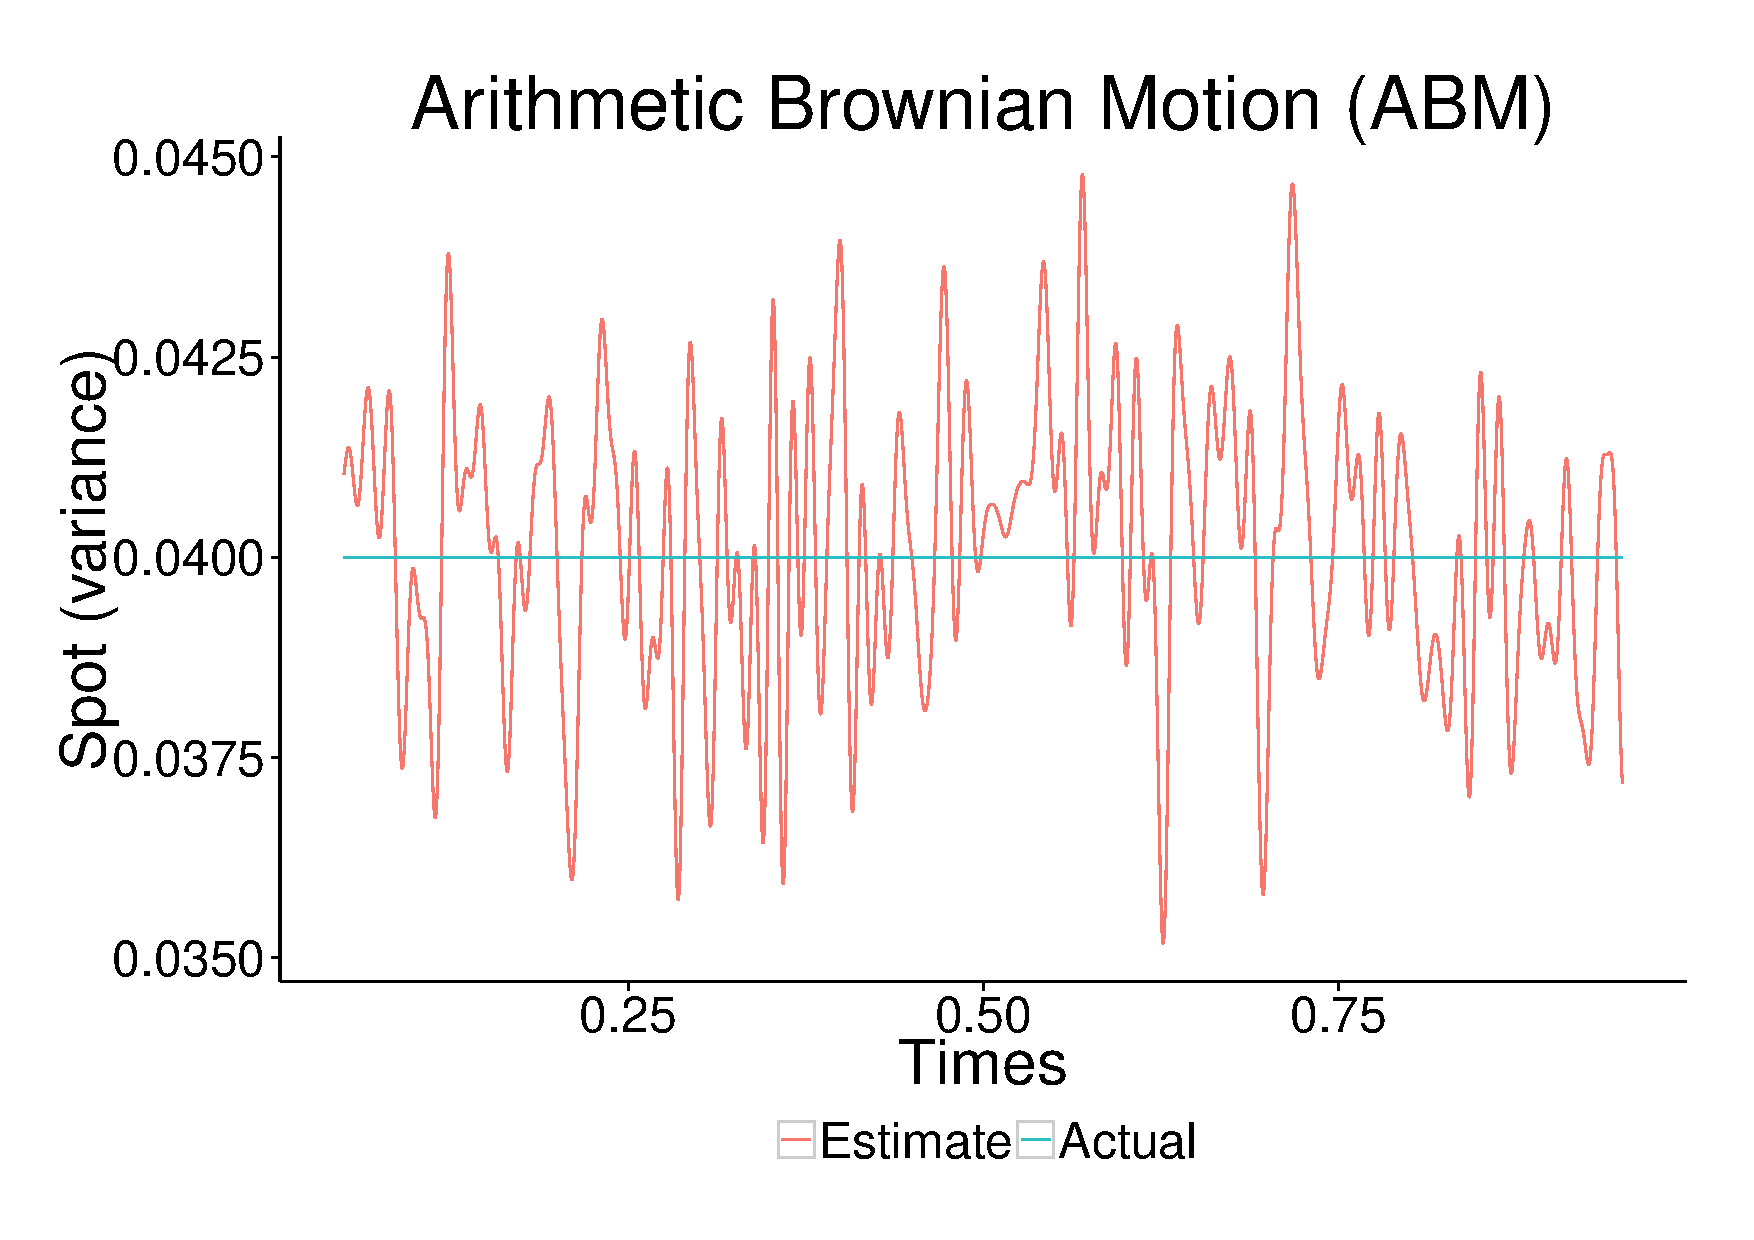
\includegraphics[angle=270,width=0.45\textwidth,totalheight=0.30\textheight]{Simulation/pa.pdf}}}
  \subfloat[GBM]{{ \includegraphics[width=0.45\textwidth]{/home/wale/Dropbox/Research/Paper3/pg.pdf}}}
  \qquad
  \subfloat[OU]{{ \includegraphics[width=0.45\textwidth]{/home/wale/Dropbox/Research/Paper3/po.pdf}}}
  \qquad
  \subfloat[ABM]{{ 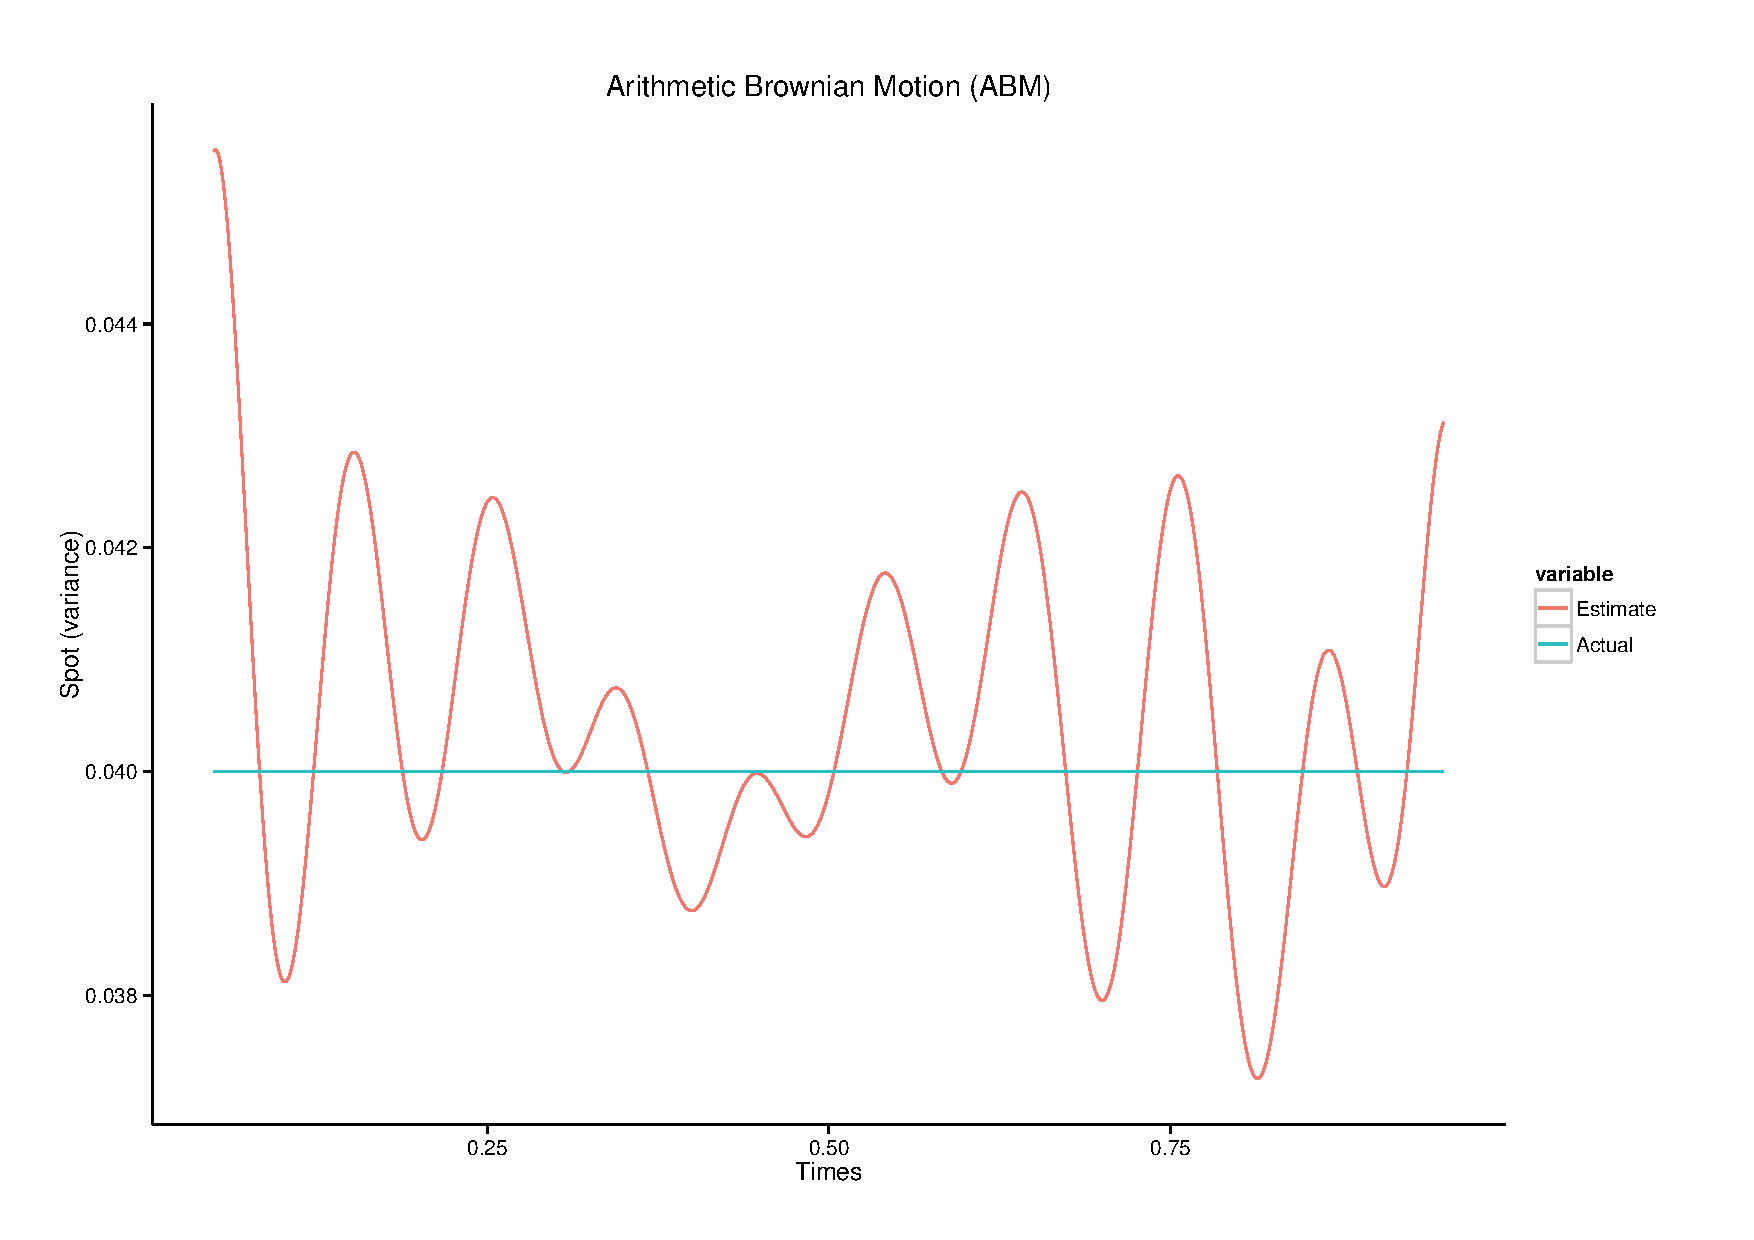
\includegraphics[width=0.45\textwidth]{/home/wale/Dropbox/Research/Paper3/pa.pdf}}}
  \subfloat[CIR]{{ 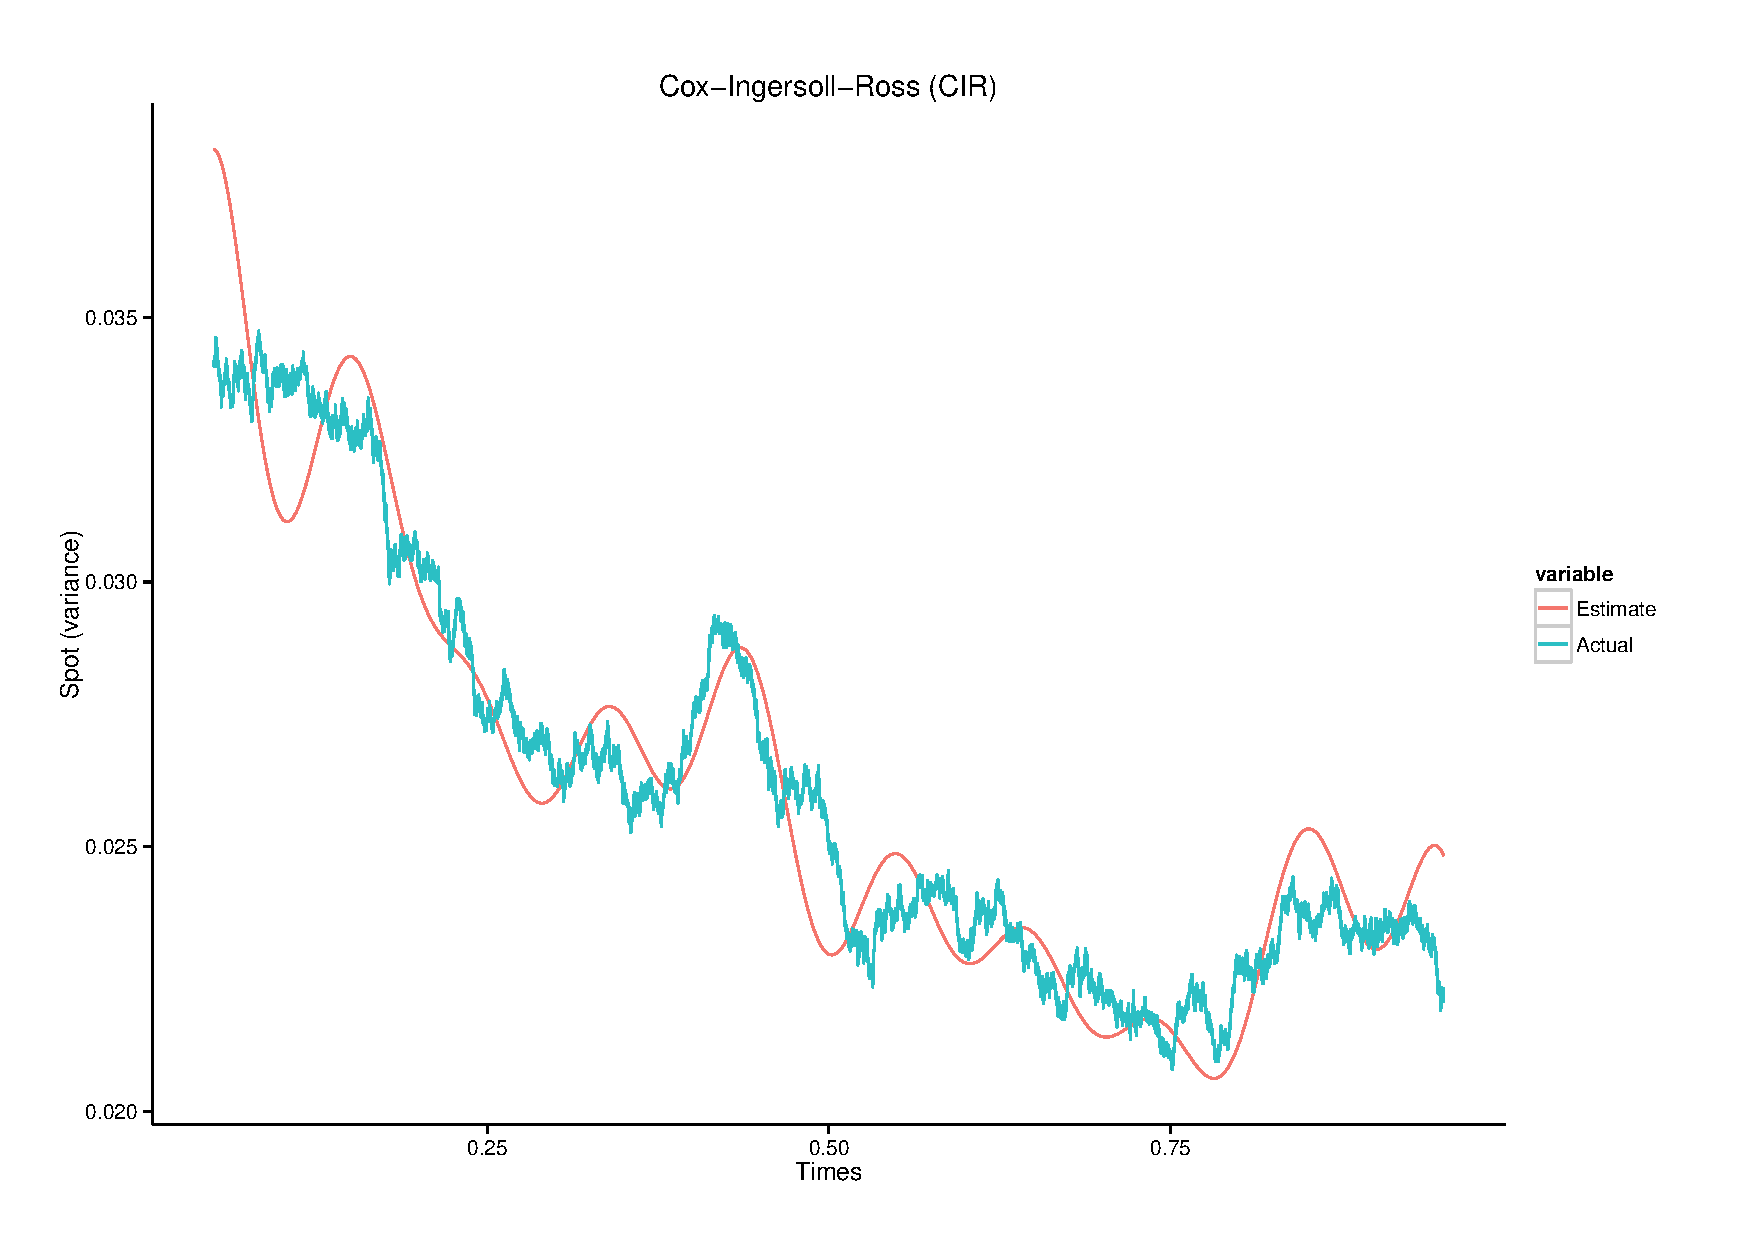
\includegraphics[width=0.45\textwidth]{/home/wale/Dropbox/Research/Paper3/pcir.pdf}}}
    \label{fig:path}
\end{figure}

\begin{landscape}
\begin{table}[ht]
  %\tabcolsep=0.11cm
\begin{threeparttable}
  %\footnotesize
%\centering
  \caption{Mean integrated square error (MISE) of $\svnx$.\label{tab:mise}}
  
\begin{tabular*} {\columnwidth}{@{\extracolsep{\stretch{1}}}*{8}{r}@{}}
    \toprule 
   & \multicolumn{3}{c}{ABM} & &\multicolumn{3}{c}{OU}\\
    \cmidrule{2-4} 
    \cmidrule{5-8} 
\multicolumn{1}{c}{$n$} & \multicolumn{1}{c}{MISE} & \multicolumn{1}{c}{Sq. Bias} & \multicolumn{1}{c}{Var} && \multicolumn{1}{c}{MISE}& \multicolumn{1}{c}{Sq. Bias} & \multicolumn{1}{c}{Var}\\
    \midrule
500 & \num[scientific-notation=true,round-precision=3,round-mode=figures]{ 0.000129690514378747 } & \num[scientific-notation=true,round-precision=3,round-mode=figures]{ 2.86098860978027e-06 } & \num[scientific-notation=true,round-precision=3,round-mode=figures]{ 0.000126829525768967 } & & \num[scientific-notation=true,round-precision=3,round-mode=figures]{ 0.000142657171197515 } & \num[scientific-notation=true,round-precision=3,round-mode=figures]{ 1.19241391058862e-05 } & \num[scientific-notation=true,round-precision=3,round-mode=figures]{ 0.000130733032091629 } \\
5000 &\num[scientific-notation=true,round-precision=3,round-mode=figures]{ 1.41480010731752e-05 } & \num[scientific-notation=true,round-precision=3,round-mode=figures]{ 1.11112511718854e-06 } & \num[scientific-notation=true,round-precision=3,round-mode=figures]{ 1.30368759559867e-05 } & & \num[scientific-notation=true,round-precision=3,round-mode=figures]{ 1.44713297500796e-05 } & \num[scientific-notation=true,round-precision=3,round-mode=figures]{ 1.62292548526195e-06 } & \num[scientific-notation=true,round-precision=3,round-mode=figures]{ 1.28484042648177e-05 } \\ 
50000 &\num[scientific-notation=true,round-precision=3,round-mode=figures]{ 2.32308652636521e-06 } & \num[scientific-notation=true,round-precision=3,round-mode=figures]{ 1.02395100012948e-06 } & \num[scientific-notation=true,round-precision=3,round-mode=figures]{ 1.29913552623573e-06 } & & \num[scientific-notation=true,round-precision=3,round-mode=figures]{ 2.35629081189399e-06 } & \num[scientific-notation=true,round-precision=3,round-mode=figures]{ 1.12403547001524e-06 } & \num[scientific-notation=true,round-precision=3,round-mode=figures]{ 1.23225534187875e-06 } \\
   \midrule
  \end{tabular*}
\end{threeparttable}
\begin{threeparttable}
  %\footnotesize
%\centering
\begin{tabular*} {\columnwidth}{@{\extracolsep{\stretch{1}}}*{8}{r}@{}}
    \midrule
   & \multicolumn{3}{c}{GBM} & &\multicolumn{3}{c}{CIR}\\
    \cmidrule{2-4} 
    \cmidrule{5-8} 
\multicolumn{1}{c}{$n$} & \multicolumn{1}{c}{MISE} & \multicolumn{1}{c}{Sq. Bias} & \multicolumn{1}{c}{Var} && \multicolumn{1}{c}{MISE}& \multicolumn{1}{c}{Sq. Bias} & \multicolumn{1}{c}{Var}\\
    \midrule
500 & \num[scientific-notation=true,round-precision=3,round-mode=figures]{ 0.000217858539705785 } & \num[scientific-notation=true,round-precision=3,round-mode=figures]{ 4.17515036941201e-06 } & \num[scientific-notation=true,round-precision=3,round-mode=figures]{ 0.000213683389336373 } && \num[scientific-notation=true,round-precision=3,round-mode=figures]{ 6.25847666534302e-05 } & \num[scientific-notation=true,round-precision=3,round-mode=figures]{ 8.51220421884097e-07 } & \num[scientific-notation=true,round-precision=3,round-mode=figures]{ 6.17335462315461e-05 } \\ 

5000 & \num[scientific-notation=true,round-precision=3,round-mode=figures]{ 2.32787518909845e-05 } & \num[scientific-notation=true,round-precision=3,round-mode=figures]{ 1.58307630511742e-06 } & \num[scientific-notation=true,round-precision=3,round-mode=figures]{ 2.16956755858671e-05 } && \num[scientific-notation=true,round-precision=3,round-mode=figures]{ 6.82420050132428e-06 } & \num[scientific-notation=true,round-precision=3,round-mode=figures]{ 5.99985785058558e-07 } & \num[scientific-notation=true,round-precision=3,round-mode=figures]{ 6.22421471626572e-06 } \\
50000 & \num[scientific-notation=true,round-precision=3,round-mode=figures]{ 4.6593085666358e-06 } & \num[scientific-notation=true,round-precision=3,round-mode=figures]{ 1.01842335658939e-06 } & \num[scientific-notation=true,round-precision=3,round-mode=figures]{ 3.64088521004641e-06 } && \num[scientific-notation=true,round-precision=3,round-mode=figures]{ 1.45783049273178e-06 } & \num[scientific-notation=true,round-precision=3,round-mode=figures]{ 6.05894054142823e-07 } & \num[scientific-notation=true,round-precision=3,round-mode=figures]{ 8.51936438588961e-07 } \\
    \bottomrule
\end{tabular*}
  \medskip
  \footnotesize
Note: The mean of the integrated square errors are obtained by taking an average over 100 sample paths generated  for each  model/number of observations pair.
\end{threeparttable}
\end{table}

\end{landscape}

From an implementation perspective, using a  B-spline  makes the construction of a \emph{dual}  frame generator a trivial matter. This is a consequence of Theorems 2.2 and 2.7 in \cite{Christensen2006}, which together specify a very simple rule for constructing  dual pairs: Let $a>0$ and $b>0$ denote  translation and modulation parameters, and let   $h$ be a B-spline of order $p$. Define the dilation operator  $\mcal{D}_c$ as follows:
\begin{align}
  \mcal{D}_c f(x) = c^{-1/2}f(x/c).  \label{eq:dilation}
\end{align}
If $0 < ab \le 1/(2 p -1)$ then  $\{\mcal{D}_a h, \mcal{D}_a\tilde{h}\}$, where 
\begin{align}
  \tilde{h}(x) = ab h(x) + 2 a b \sum^{p-1}_{n=1} h(x+n), \qquad  x \in \real, 
  \label{eq:gt}
\end{align}
is a pair of  dual Gabor  frame generators. So if we start with a B-spline $h$ then the dual generator will be a finite linear combination of scaled translates of $h$; consequently, the  dual generator will be a spline, with similar regularity properties.  For our simulation, we used a third-order B-spline. Our choice of the third order B-spline is motivated by a desire for a generator with a  Fourier transform that decays like a quadratic polynomial.   Specifically, we set
\begin{align}
  h(x) = \left\{
    \begin{array}{lr}
    x^2/2 & x \in (1,0]\\
  (-2x^2 + 6x - 3)/2 & x \in (2,1]\\
(3-x^2)/2 & x \in (3,2]\\
0 & x \not\in (3,0]
\end{array}\right. ,
  \label{eq:theh}
\end{align}
with  $\tilde{h}$ computed as in \eqref{eq:gt} above.
Our choice of the modulation and translation parameters is rather arbitrary. The only constraint is that $0 < ab \le 1/(2p -1) = 1/5$; from our experimentation with different values, performance seems to be about the same for different choices satisfying the inequality;  we settled on $a = 1/5$ and $b = 1/3$.  Ideally $H_n$, the order of the number of frequency domain shifts, would be selected optimally to minimize MISE while balancing integrated variance and integrated square  bias; this is an open research question. For the time being we  set $H_n$ naively equal to 50.

The simulation results indicate that the Gabor frame estimator performs satisfactorily. Figure~\ref{fig:path} displays, for each of the 4 price models (ABM, OU, GBM, and CIR), simulated  spot variance sample paths plotted against spot variance paths produced by the Gabor frame estimator.  A visual inspection shows that the estimator produces a relatively good fit even with the naive selection of $H_n$. This claim is further corroborated by the analysis of the the \mise (MISE), the \isqb, and the \ivar summarized in Table \ref{tab:mise}.\begin{comment} 
The figures in the table are arrived at in the following manner: first,  100 price histories are simulated for each observation frequency and  model pair.  So, each history is the result of sampling $n$ price observations from  distribution $F$, where $n$ is the specified observation frequency and $F$ is the distribution implied by the stochastic differential equation. The resulting data is a matrix with 100 rows and $n$ columns.  Each row represents a price history from which integrated quatities may be obatined, and each column indexes an orbservation time. Going down a column, average quantities may be computed. 
For instance, to arrive at the integrated square bias figures, average spot variances were computed for each observation times; the figures were then squared, weighted by $\Delta_n$, and summed up. The integrated mean square error is computed similarly. \end{comment}
 We found that the variance, estimated in the foregoing manner,  is only approximately the difference between the MISE and the integrated square bias.  The reported figures for variance are  in fact the difference between the MISE and the integrated square bias. The discrepancy is rather slight and does not materially change the result. In all 4 model, an inverse relation between MISE, square bias, and variance may be read off from the table. As was established mathematically, we expect MISE to vanish if the number of price observations were made to grow without bound.    
 \subsection{Prices with jumps}
We continue our investigation by simulating prices with jumps.    
\begin{align}
  & X_t = 0.8 +  0.5  t + 0.2  W_t + \sum_{i = 1}^N Y_i,\notag & \text{(ABM + JMP)}\\
  & X_t = 0.8 -\int_0^t 4 X_s \D s + \int^t_0 0.2 \D W_s +  \sum_{i = 1}^N Y_i ,\notag & \text{(OU + JMP)}\\
  & X_t = 0.8 + \int_0^t 0.5 X_s \D s + \int^t_0 0.2 X_s \D W_s + \sum_{i = 1}^N Y_i,\notag & \text{(GBM + JMP)}\\
  & X_t = 0.8 + \int_0^t(0.1 - 0.5 X_s) \D s +\int^t_0  0.2 \sqrt{X_s} \D W_s + \sum_{i = 1}^N Y_i,\notag & \text{(CIR + JMP)}
  \label{}
\end{align}
wher $N$ is a Poisson random variable with intensity $5$ and $Y_i$, $1 \le  i\le N$, is a normal random variable with mean zero and standard deviation 0.4.  

We construct the dual  Gabor frames as in the previous subsection using the  third order B-Spline specified in \eqref{eq:theh}. With the introduction of jumps into the simulation, we found out that better results may be obtained by varying tha parameters $a,b,$ and $H_n$. We settled on $a = 1/7$, $b = 1/25$, and $H_n = 50$. The jump threshold is obtained by setting $u_n = n^{\alpha}$, where $\alpha = -0.9$. The results of the simulations are recorded in Table~\ref{tab:misej}. We also produce a graph of a single observations (paths) in Figure~\ref{fig:pathj}. %It is apparent from this simulation study that, eventhough the analytical part of the analysis assumed that volatility is continuous, the estimator \jvn works fine in cases where volatiity is \cadlag. This is the case when we add jumps to the geometric Brownian  and the CIR processes. We defer an analytical study of this more general situation to future work.
\begin{figure}
  \caption{Estimated vs. actual spot volatility of common price models}
  \centering
  %\subfloat[ABM]{{ 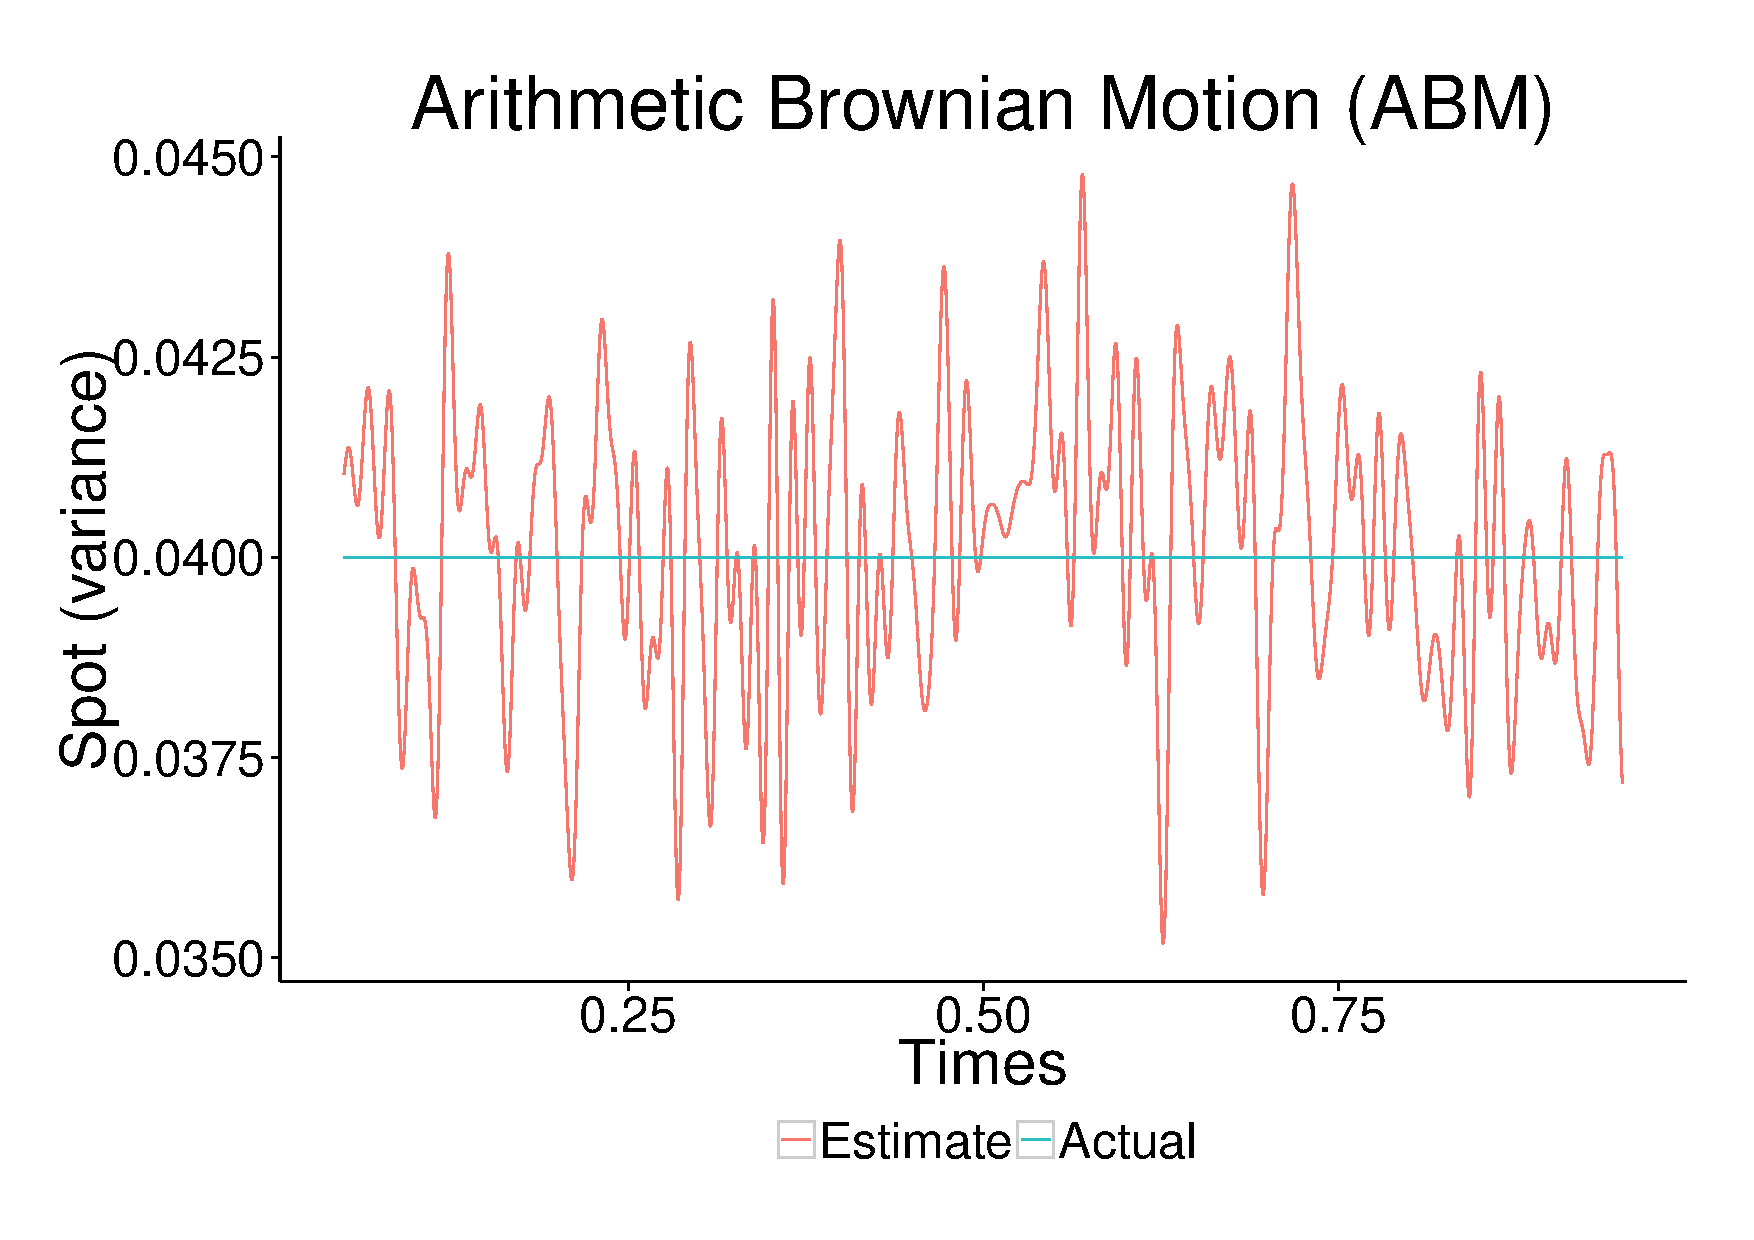
\includegraphics[angle=270,width=0.45\textwidth,totalheight=0.30\textheight]{Simulation/pa.pdf}}}
  \subfloat[GBM + JMP]{{ \includegraphics[width=0.45\textwidth]{/home/wale/Dropbox/Research/Paper3/Simulation/pg.pdf}}}
  \qquad
  \subfloat[OU + JMP]{{ \includegraphics[width=0.45\textwidth]{/home/wale/Dropbox/Research/Paper3/Simulation/po.pdf}}}
\qquad
  \subfloat[ABM]{{ 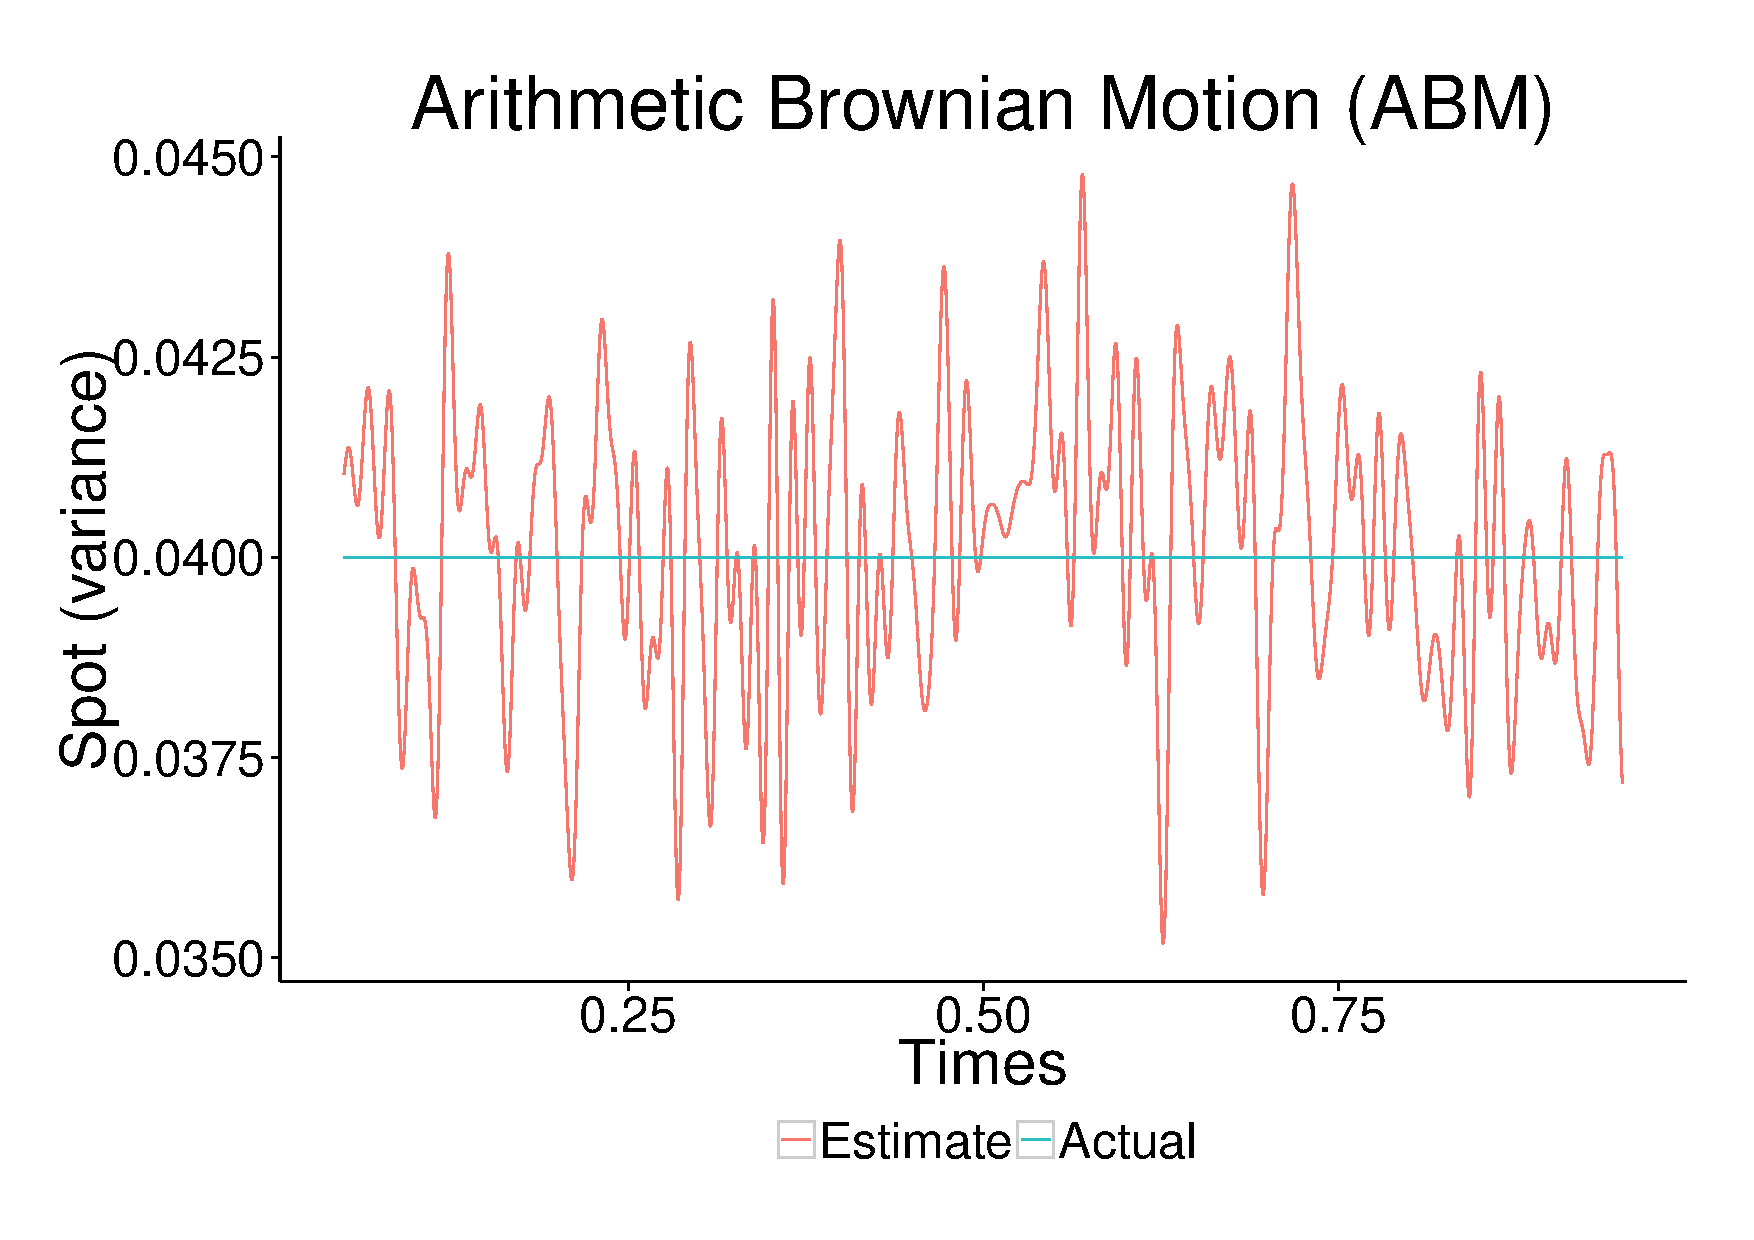
\includegraphics[angle=270,width=0.45\textwidth,totalheight=0.30\textheight]{Simulation/pa.pdf}}}
%  \subfloat[GBM+JUMP]{{ 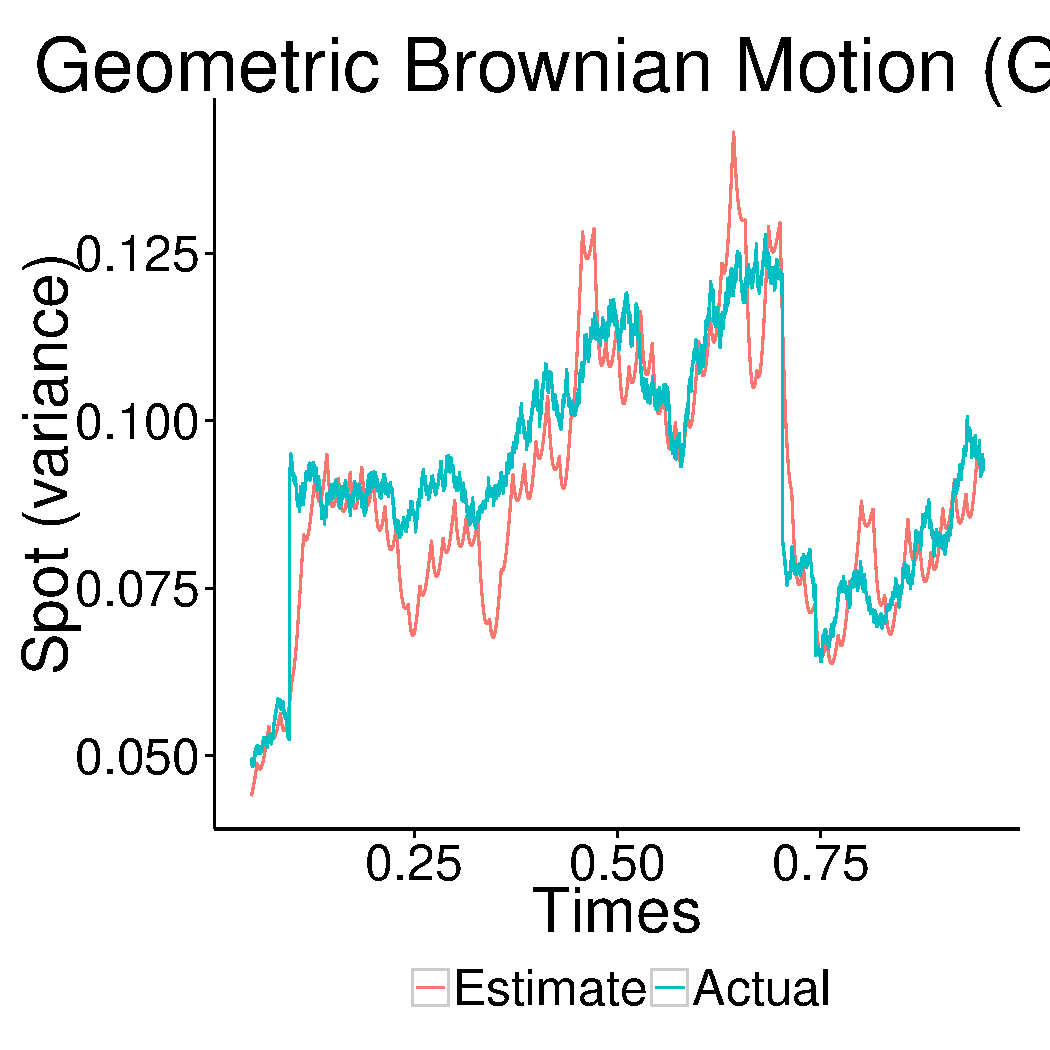
\includegraphics[width=0.45\textwidth]{/home/wale/Dropbox/Research/Paper3/Simulation/bpg.pdf}}}
  \qquad
  \subfloat[CIR+JUMP]{{ 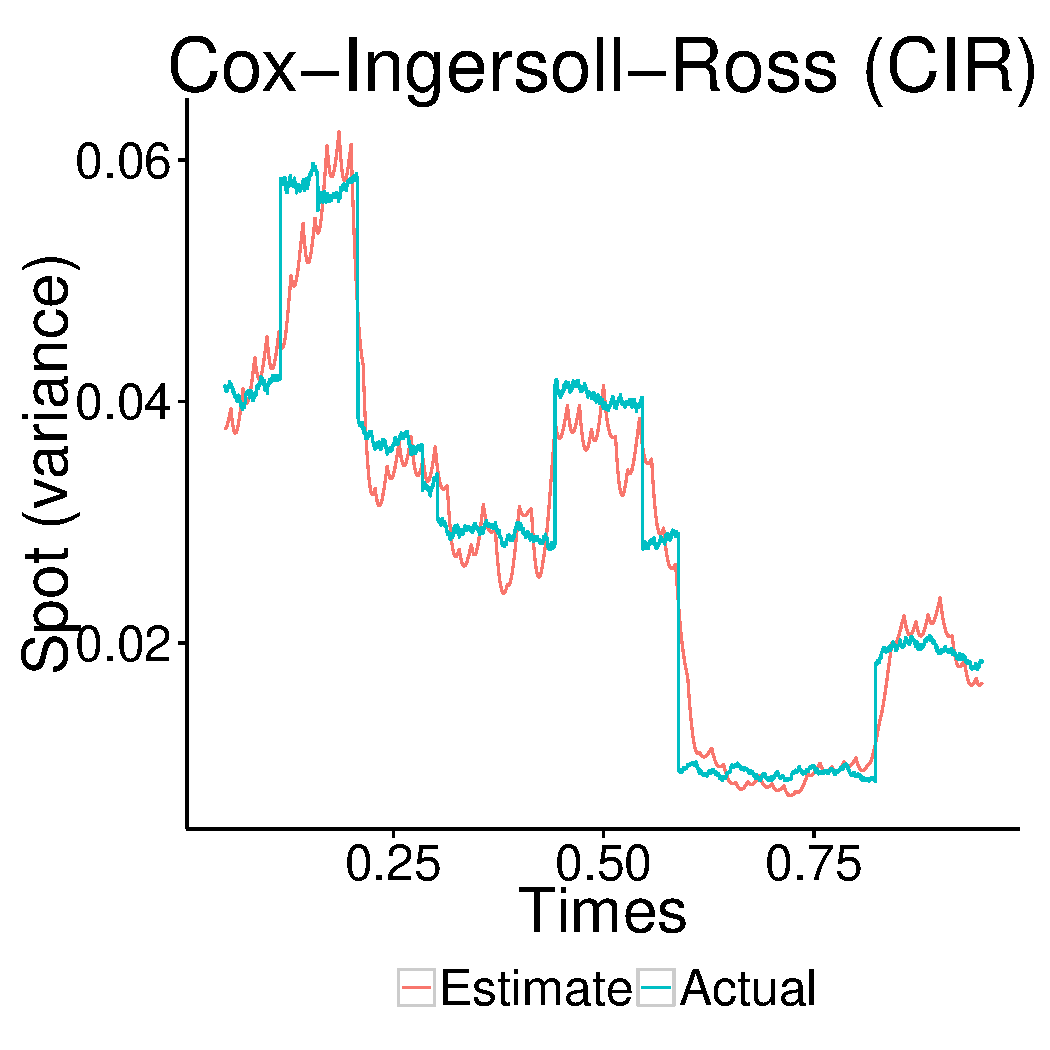
\includegraphics[width=0.45\textwidth]{/home/wale/Dropbox/Research/Paper3/Simulation/bpc.pdf}}}
    \label{fig:path}
\end{figure}

\begin{table}[ht]
  %\tabcolsep=0.11cm
\begin{threeparttable}
  %\footnotesize
%\centering
  \caption{Mean integrated square error (MISE) of the frame-based estimator $\hat{\sigma}_n^2$ for popular price models.\label{tab:mise}}
  
\begin{tabular*} {\columnwidth}{@{\extracolsep{\stretch{1}}}*{8}{r}@{}}
    \toprule 
   & \multicolumn{3}{c}{FP} & &\multicolumn{3}{c}{OU}\\
    \cmidrule{2-4} 
    \cmidrule{5-8} 
\multicolumn{1}{c}{$n$} & \multicolumn{1}{c}{MISE} & \multicolumn{1}{c}{Sq. Bias} & \multicolumn{1}{c}{Var} && \multicolumn{1}{c}{MISE}& \multicolumn{1}{c}{Sq. Bias} & \multicolumn{1}{c}{Var}\\
    \midrule
500 & \num[scientific-notation=true,round-precision=3,round-mode=figures]{ 0.000152943970286857 } & \num[scientific-notation=true,round-precision=3,round-mode=figures]{ 8.95426446735699e-06 } & \num[scientific-notation=true,round-precision=3,round-mode=figures]{ 0.0001439897058195 } && \num[scientific-notation=true,round-precision=3,round-mode=figures]{ 0.0008507085185364 } & \num[scientific-notation=true,round-precision=3,round-mode=figures]{ 0.000130637321821816 } & \num[scientific-notation=true,round-precision=3,round-mode=figures]{ 0.000720071196714584 } \\ 
5000 & \num[scientific-notation=true,round-precision=3,round-mode=figures]{ 2.18676452382767e-05 } & \num[scientific-notation=true,round-precision=3,round-mode=figures]{ 2.27386491244051e-06 } &  \num[scientific-notation=true,round-precision=3,round-mode=figures]{ 1.95937803258361e-05 } && \num[scientific-notation=true,round-precision=3,round-mode=figures]{ 5.47538962275779e-05 } & \num[scientific-notation=true,round-precision=3,round-mode=figures]{ 9.75968033436806e-06 } & \num[scientific-notation=true,round-precision=3,round-mode=figures]{ 4.49942158932098e-05 } \\ 
50000 & \num[scientific-notation=true,round-precision=3,round-mode=figures]{ 2.1312724152077e-06 } & \num[scientific-notation=true,round-precision=3,round-mode=figures]{ 8.9974544209342e-08 } & \num[scientific-notation=true,round-precision=3,round-mode=figures]{ 2.04129787099836e-06 } && \num[scientific-notation=true,round-precision=3,round-mode=figures]{ 6.6114774335773e-06 } & \num[scientific-notation=true,round-precision=3,round-mode=figures]{ 2.64501211826553e-06 } & \num[scientific-notation=true,round-precision=3,round-mode=figures]{ 3.96646531531177e-06 } \\
   \midrule
  \end{tabular*}
\end{threeparttable}
\begin{threeparttable}
  %\footnotesize
%\centering
\begin{tabular*} {\columnwidth}{@{\extracolsep{\stretch{1}}}*{8}{r}@{}}
    \midrule
   & \multicolumn{3}{c}{GBM} & &\multicolumn{3}{c}{CIR}\\
    \cmidrule{2-4} 
    \cmidrule{5-8} 
\multicolumn{1}{c}{$n$} & \multicolumn{1}{c}{MISE} & \multicolumn{1}{c}{Sq. Bias} & \multicolumn{1}{c}{Var} && \multicolumn{1}{c}{MISE}& \multicolumn{1}{c}{Sq. Bias} & \multicolumn{1}{c}{Var}\\
    \midrule


500 & \num[scientific-notation=true,round-precision=3,round-mode=figures]{ 0.00613398704893088 } & \num[scientific-notation=true,round-precision=3,round-mode=figures]{ 0.000870352351606066 } & \num[scientific-notation=true,round-precision=3,round-mode=figures]{ 0.00526363469732481 } && \num[scientific-notation=true,round-precision=3,round-mode=figures]{ 0.000374450452612452 } & \num[scientific-notation=true,round-precision=3,round-mode=figures]{ 0.000231573404584565 } & \num[scientific-notation=true,round-precision=3,round-mode=figures]{ 0.000142877048027886 } \\ 
5000 & \num[scientific-notation=true,round-precision=3,round-mode=figures]{ 0.000342385006317484 } & \num[scientific-notation=true,round-precision=3,round-mode=figures]{ 4.07189648661911e-05 }  &\num[scientific-notation=true,round-precision=3,round-mode=figures]{ 0.000301666041451293 } && \num[scientific-notation=true,round-precision=3,round-mode=figures]{ 1.12423351227354e-05 } & \num[scientific-notation=true,round-precision=3,round-mode=figures]{ 8.2888360643758e-06 } & \num[scientific-notation=true,round-precision=3,round-mode=figures]{ 2.95349905835962e-06 } \\ 
50000 & \num[scientific-notation=true,round-precision=3,round-mode=figures]{ 7.10632627767849e-05 } & \num[scientific-notation=true,round-precision=3,round-mode=figures]{ 6.36155753555274e-06 } & \num[scientific-notation=true,round-precision=3,round-mode=figures]{ 6.47017052412321e-05 } && \num[scientific-notation=true,round-precision=3,round-mode=figures]{ 7.04582898194268e-06 } & \num[scientific-notation=true,round-precision=3,round-mode=figures]{ 5.64425630312442e-06 } & \num[scientific-notation=true,round-precision=3,round-mode=figures]{ 1.40157267881827e-06 } \\
    \bottomrule
\end{tabular*}
  \medskip
  \footnotesize
Note: The mean of the integrated square errors are obtained by taking an average over 50 sample paths generated  for each  model/number of observations pair.
\end{threeparttable}
\end{table}


